\section{KDD99数据集处理}

\subsection{KDD99数据集简介}
KDD99数据集是模拟数据集,模拟美国空军局域网搜集的大概九周的网络连接数据,可分为两部分:带有标识的训练数据、未加标识的测试数据。为了检测数据模型,测试数据中包含了训练数据中没有的数据类型,以便更接近真实的入侵检测。本次实验采用KDD99的训练数据集。
正常识别类型和22种训练攻击类型包含在训练数据集中,如图所示。 此外,有14种攻击仅出现在测试数据集中而不在训练集中。



\begin{table}[h]\wuhao
	\centering  %作用是使表格居中
	\caption{训练数据集标识类型1} 
	\label{}
	\begin{spacing}{1.35}  %调整表格行距
	\begin{tabular}{p{3cm}<{\raggedright}p{4cm}<{\raggedright}p{6cm}<{\raggedright}}
		\hline
		标识类型    & 含义                 & 具体分类标识                                                                 \\ \hline
		Normal  & 正常记录               & Normal                                                                 \\
		DOS     & 拒绝服务攻击             & back、land、neptune、pod、smurf、teardrop                                   \\
		Probing & 监视和其他探测活动          & ipsweep、nmap、portsweep、satan                                           \\
		R2L     & 来自远程机器的非法访问        & ftp\_write、guess\_passwd、imap、multihop、phf、spy、warezclient、warezmaster \\
		U2R     & 普通用户对本地超级用户特权的非法访问 & buffer\_overflow、loadmodule、perl、rootkit                               \\ \hline
	\end{tabular} 
	\end{spacing}
\end{table}


\begin{table}[h]
	\centering
	\caption{训练数据集标识类型2}
	\label{}
	\begin{spacing}{1.35}  %调整表格行距 
	\begin{tabular}{@{}llll@{}}
		\toprule
		标签 & 类别     & 训练集(10\%) & 测试集(Corrected) \\ \midrule
		0  & NORMAL & 97278     & 60593         
	\end{tabular}
	\end{spacing}
\end{table}



\begin{figure}[h]  % [h]排版时把图片放在当前位置
	\centering
	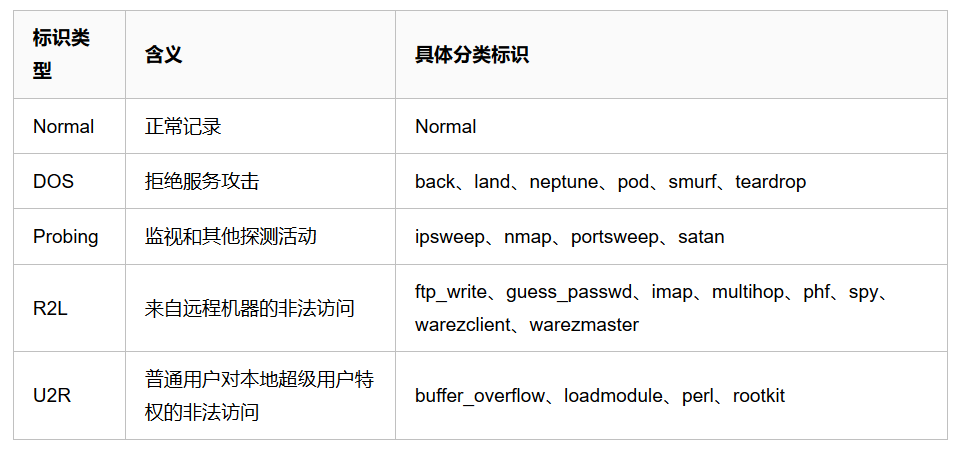
\includegraphics[width=0.98\textwidth]{fig_03_01.png}
	\caption{训练数据集标识类型}
	\label{}
\end{figure}
数据特征:KDD99训练数据集中有42维特征,其中前41维特征是连接记录的固定特征,最后一维是类标识符,用于指示连接记录是正常还是特定攻击类型。 在前41维特征中,9个特征属性是离散的数据,而其他属性是连续的数据。如下图3-2所示。

\begin{figure}[h]
	\centering
	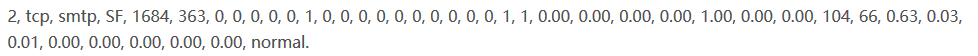
\includegraphics[width=0.98\textwidth]{fig_03_02.png}
	\caption{KDD99训练数据集}
	\label{}
\end{figure}

\subsection{数据预处理}
\subsubsection{观察数据}
\subsubsection{离散型数据预处理}
离散数据,也称字符型数据。计算机不能直接处理字符型数据,因此我们需要在算法开始之前对数据进行一系列的特征处理、转换。

针对KDD99数据集中的四类字符型数据做如下处理:

\subsubsection{连续型数据预处理}
	\begin{enumerate}  
		\item 设置变量X为数据集,变量Y为标签:
			
			\begin{figure}[h]  % [h]排版时把图片放在当前位置  浮动体就放在当前页面上,适合小浮动体
				\centering
				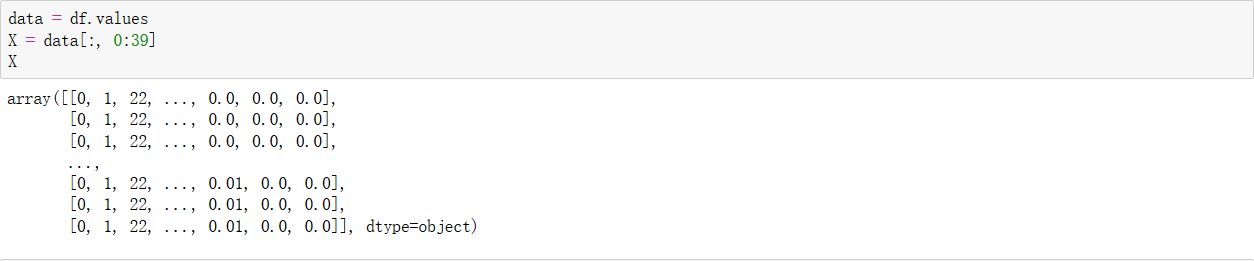
\includegraphics[width=0.98\textwidth]{fig_03_17.png}
				\caption{数据集X}
				\label{}
			\end{figure}
			\begin{figure}[h]  % [h]排版时把图片放在当前位置
				\centering
				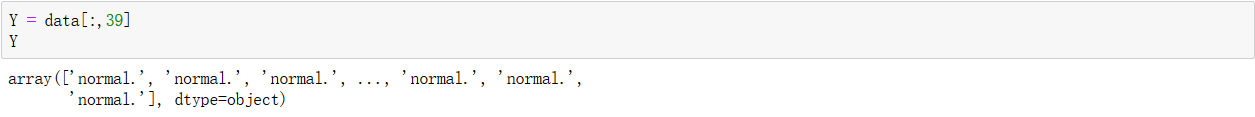
\includegraphics[width=0.98\textwidth]{fig_03_18.png}
				\caption{数据集Y}
				\label{}
			\end{figure}
		\item 设置变量X为数据集,变量Y为标签:
			
			进行数据标准化的原因:对于同一个特征来说,不同的样本中的取值有可能会相差很常大,一些异常的数据会误导模型的正确训练;除此之外,如果数据的分布很分散也会影响训练结果。以上两种数据的数据方差会非常大。此时,我们可以将特征中的值进行标准差标准化,即转换为均值为0,方差为1的正态分布。
	
			其原理是 
			$$x^{*}=\frac{x-\overline{x}}{\sigma}$$  % 单独占一行,mathpix
			其中,$x^*$为原始数据的均值,$\sigma$为原始数据的标准差。$\sigma$反应了给定数据距离其均值标准差的大小,高于平均值的数据将获得正标准化分数,反之亦然将获得负标准化分数。
			
			本实验使用python中的sklearn.preprocessing.StandardScaler类,通过
			StandardScaler模块计算标准化。标准化数据如下:
			\begin{figure}[h]  % [h]排版时把图片放在当前位置
				\centering
				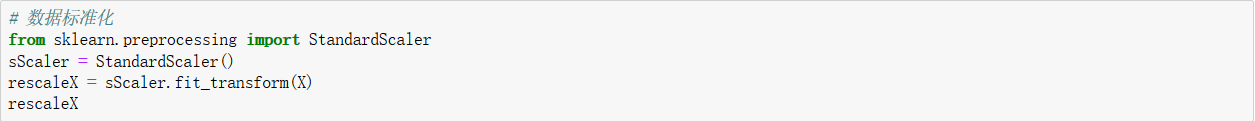
\includegraphics[width=0.98\textwidth]{fig_03_19.png}
				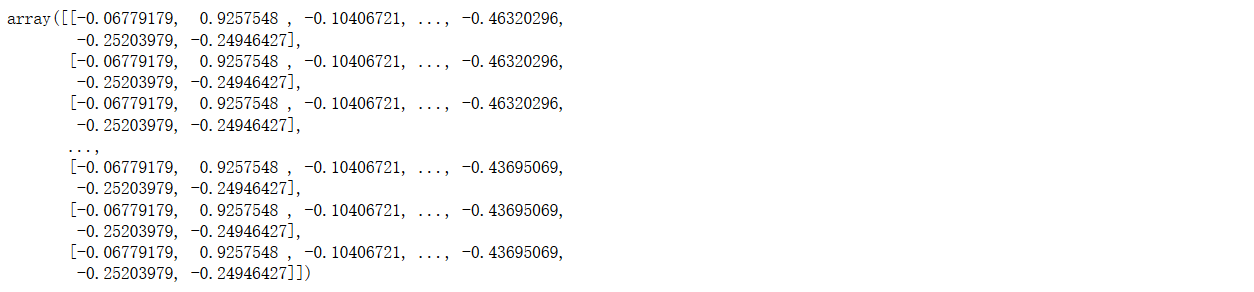
\includegraphics[width=0.98\textwidth]{fig_03_19_2.png}
				\caption{标准化后的数据}
				\label{}
			\end{figure}

		\item 对数据进行归一化:
		
			进行数据归一化的原因:拿到数据样本时,数据的单位往往不一致,在计算期间将数据缩放到特定间隔。处理用于比较和评估的指标时,可以将数据的单位限制去除并且将其转换为无量纲值,从而比较和加权不同单位或大小的指标。


	\end{enumerate} 

	 
	


\subsubsection{特征降维}
\begin{figure}[h]  % [h]排版时把图片放在当前位置
	\centering
	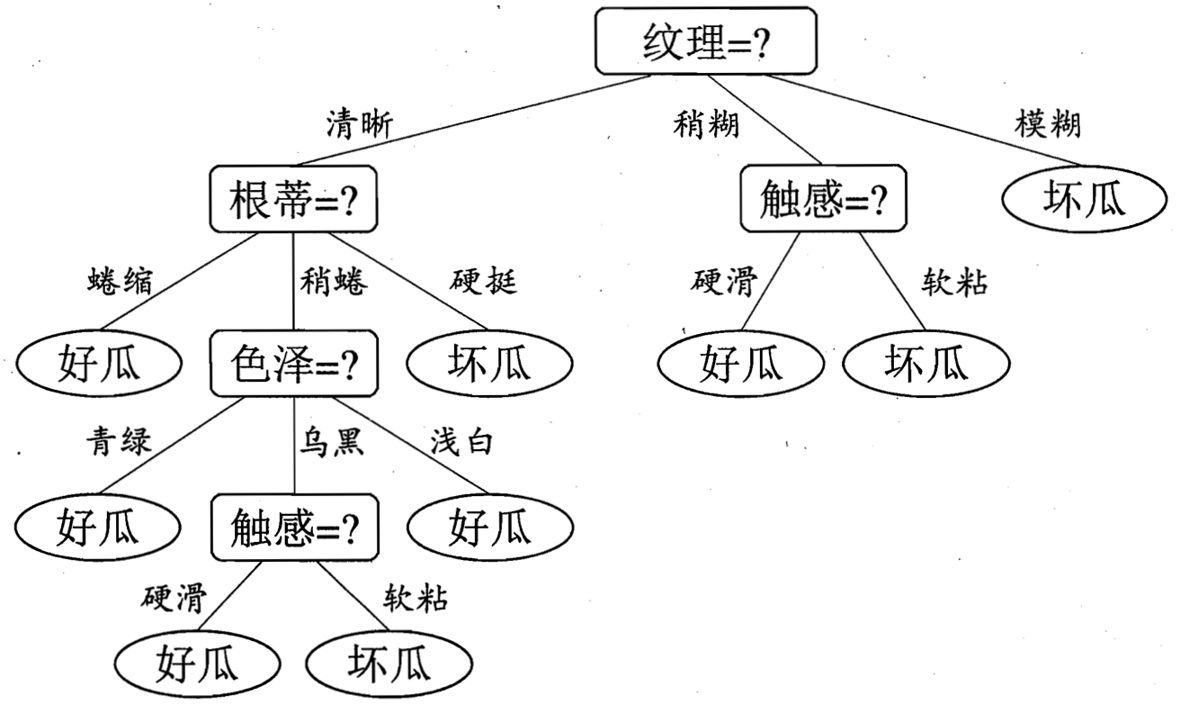
\includegraphics[width=0.98\textwidth]{fig_03_22.jpg}
	\caption{西瓜书}
	%\label{fig:1} % label放在caption之后,格式:书签名:类型:类名
	\label{}
\end{figure}

西瓜书 \footnote{周志华,《机器学习》}中写道:
\begin{quotation}
{\kaishu 归纳(induction)和演绎(deduction)是科学推理的两大基本手段,归纳是从特殊到一般的“泛化”(generation)的过程}	
\end{quotation}



\subsection{本章小结}
总结一下。

\setcounter{table}{0}  % 表格编号置0
\setcounter{figure}{0} % 图片编号置0
\setcounter{equation}{0} % 方程号置0